\documentclass[main.tex]{subfiles} % Subfile-Class


% ============================================================================== %
%                            Subfile document                                    %
% ============================================================================== %

\begin{document}

\begin{landscape} % Querformat beginnen
    \thispagestyle{fancy}

    \subsection{Nutzwertanalyse Pfadfinder}

    \begin{table}[ht]
        \centering
        \begin{tabular}{|p{0.11\linewidth}|p{0.18\linewidth}|p{0.085\linewidth}|p{0.057\linewidth}|p{0.07\linewidth}|p{0.057\linewidth}|p{0.07\linewidth}|p{0.057\linewidth}|p{0.07\linewidth}|}
            \hline
                                                      &                                     &                                            &                                           &                                            &            &             &            &             \\[-9pt]
                                                      & \multirow{2}{*}{\textbf{Kriterien}} & Gewichtung                                 & Punkte                                    & Punkte                                     & Punkte     & Punkte      & Punkte     & Punkte      \\[1pt]
                                                      &                                     & \{\%\}                                     & \{1...10\}                                & gewichtet                                  & \{1...10\} & gewichtet   & \{1...10\} & gewichtet   \\[1pt]
            \hline
            \hline
                                                      & \multicolumn{2}{c|}{}               & \multicolumn{2}{c|}{}                      & \multicolumn{2}{c|}{}                     & \multicolumn{2}{c|}{}                                                                            \\[-9pt]
            \multirow{7}{4em}{\textbf{Gesamt-system}} & \multicolumn{2}{c|}{}               & \multicolumn{2}{c|}{\textbf{rote Linie}}   & \multicolumn{2}{c|}{\textbf{grüne Linie}} & \multicolumn{2}{c|}{\textbf{blaue Linie}}                                                        \\[1pt]
            \cline{2-9}
                                                      &                                     &                                            &                                           &                                            &            &             &            &             \\[-9pt]
                                                      & Einrichtungsaufwand                 & 15                                         & 8                                         & 12                                         & 5          & 7.5         & 6          & 9           \\[1pt]
            \cline{2-9}
                                                      &                                     &                                            &                                           &                                            &            &             &            &             \\[-9pt]
                                                      & Entwicklungsaufwand                 & 25                                         & 6                                         & 15                                         & 3          & 7.5         & 8          & 20          \\[1pt]
            \cline{2-9}
                                                      &                                     &                                            &                                           &                                            &            &             &            &             \\[-9pt]
                                                      & Geschwindigkeit                     & 20                                         & 7                                         & 14                                         & 5          & 10          & 9          & 18          \\[1pt]
            \cline{2-9}
                                                      &                                     &                                            &                                           &                                            &            &             &            &             \\[-9pt]
                                                      & Kosten                              & 30                                         & 8                                         & 24                                         & 4          & 12          & 6          & 18          \\[1pt]
            \cline{2-9}
                                                      &                                     &                                            &                                           &                                            &            &             &            &             \\[-9pt]
                                                      & Nachhaltigkeit                      & 10                                         & 5                                         & 5                                          & 3          & 3           & 4          & 4           \\[1pt]
            \cline{2-9}
                                                      &                                     &                                            &                                           &                                            &            &             &            &             \\[-9pt]
                                                      & \textbf{Summe}                      & \textbf{100}                               &                                           & \textbf{70}                                &            & \textbf{40} &            & \textbf{69} \\[1pt]
            \hline
            \hline
                                                      & \multicolumn{2}{c|}{}               & \multicolumn{2}{c|}{}                      & \multicolumn{2}{c|}{}                     & \multicolumn{2}{c|}{}                                                                            \\[-9pt]
            \multirow{6}{4em}{\textbf{Antrieb}}       & \multicolumn{2}{c|}{}               & \multicolumn{2}{c|}{\textbf{Schrittmotor}} & \multicolumn{2}{c|}{\textbf{DC-Motor}}    & \multicolumn{2}{c|}{\textbf{Schrittmotor}}                                                       \\[1pt]
            \cline{2-9}
                                                      &                                     &                                            &                                           &                                            &            &             &            &             \\[-9pt]
                                                      & Geschwindigkeit                     & 20                                         & 8                                         & 16                                         & 8          & 16          & 8          & 16          \\[1pt]
            \cline{2-9}
                                                      &                                     &                                            &                                           &                                            &            &             &            &             \\[-9pt]
                                                      & Verhältnis Leistung zu Gewicht      & 30                                         & 4                                         & 12                                         & 7          & 21          & 4          & 12          \\[1pt]
            \cline{2-9}
                                                      &                                     &                                            &                                           &                                            &            &             &            &             \\[-9pt]
                                                      & Wendefähigkeit                      & 20                                         & 8                                         & 16                                         & 10         & 20          & 8          & 16          \\[1pt]
            \cline{2-9}
                                                      &                                     &                                            &                                           &                                            &            &             &            &             \\[-9pt]
                                                      & Genauigkeit                         & 30                                         & 7                                         & 21                                         & 4          & 12          & 7          & 21          \\[1pt]
            \cline{2-9}
                                                      &                                     &                                            &                                           &                                            &            &             &            &             \\[-9pt]
                                                      & \textbf{Summe}                      & \textbf{100}                               &                                           & \textbf{65}                                &            & \textbf{69} &            & \textbf{65} \\[1pt]
            \hline

        \end{tabular}
        \caption{Nutzwertanalyse Pfadfinder 1}
    \end{table}

    \newpage
    \begin{table}[ht]
        \centering
        \begin{tabular}{|p{0.11\linewidth}|p{0.18\linewidth}|p{0.085\linewidth}|p{0.057\linewidth}|p{0.07\linewidth}|p{0.057\linewidth}|p{0.07\linewidth}|p{0.057\linewidth}|p{0.07\linewidth}|}
            \hline
                                                           & \multicolumn{2}{c|}{}               & \multicolumn{2}{c|}{}                      & \multicolumn{2}{c|}{}                       & \multicolumn{2}{c|}{}                                                             \\[-9pt]
            \multirow{6}{4em}{\textbf{Hindernis-handling}} & \multicolumn{2}{c|}{}               & \multicolumn{2}{c|}{\textbf{Greifer ohne}} & \multicolumn{2}{c|}{\textbf{Gabelstapler}}  & \multicolumn{2}{c|}{\textbf{Greifer mit}}                                         \\[1pt]
                                                           & \multicolumn{2}{c|}{}               & \multicolumn{2}{c|}{\textbf{Ausrichtung}}  & \multicolumn{2}{c|}{\textbf{}}              & \multicolumn{2}{c|}{\textbf{Ausrichtung}}                                         \\[1pt]
            \cline{2-9}
                                                           &                                     &                                            &                                             &                                             &   &               &   &             \\[-9pt]
                                                           & Platziergenauigkeit                 & 25                                         & 7                                           & 17.5                                        & 4 & 10            & 8 & 20          \\[1pt]
            \cline{2-9}
                                                           &                                     &                                            &                                             &                                             &   &               &   &             \\[-9pt]
                                                           & Sicherheit                          & 45                                         & 6                                           & 27                                          & 7 & 31.5          & 6 & 27          \\[1pt]
            \cline{2-9}
                                                           &                                     &                                            &                                             &                                             &   &               &   &             \\[-9pt]
                                                           & Robustheit                          & 30                                         & 8                                           & 24                                          & 7 & 21            & 6 & 18          \\[1pt]
            \cline{2-9}
                                                           &                                     &                                            &                                             &                                             &   &               &   &             \\[-9pt]
                                                           & \textbf{Summe}                      & \textbf{100}                               &                                             & \textbf{68.5}                               &   & \textbf{62.5} &   & \textbf{65} \\[1pt]
            \hline
            \hline
                                                           & \multicolumn{2}{c|}{}               & \multicolumn{2}{c|}{}                      & \multicolumn{2}{c|}{}                       & \multicolumn{2}{c|}{}                                                             \\[-9pt]
            \multirow{4}{4em}{\textbf{Energie-versorgung}} & \multicolumn{2}{c|}{}               & \multicolumn{2}{c|}{\textbf{Li-ion Akku}}  & \multicolumn{2}{c|}{\textbf{Ni-Cd Akku}}    & \multicolumn{2}{c|}{\textbf{Li-ion Akku}}                                         \\[1pt]
            \cline{2-9}
                                                           &                                     &                                            &                                             &                                             &   &               &   &             \\[-9pt]
                                                           & Laufzeit                            & 40                                         & 9                                           & 36                                          & 7 & 28            & 9 & 36          \\[1pt]
            \cline{2-9}
                                                           &                                     &                                            &                                             &                                             &   &               &   &             \\[-9pt]
                                                           & Gewicht                             & 60                                         & 9                                           & 54                                          & 7 & 42            & 9 & 54          \\[1pt]
            \cline{2-9}
                                                           &                                     &                                            &                                             &                                             &   &               &   &             \\[-9pt]
                                                           & \textbf{Summe}                      & \textbf{100}                               &                                             & \textbf{90}                                 &   & \textbf{70}   &   & \textbf{90} \\[1pt]
            \hline
            \hline
                                                           & \multicolumn{2}{c|}{}               & \multicolumn{2}{c|}{}                      & \multicolumn{2}{c|}{}                       & \multicolumn{2}{c|}{}                                                             \\[-9pt]
            \multirow{6}{4em}{\textbf{Umwelt-detektion}}   & \multicolumn{2}{c|}{}               & \multicolumn{2}{c|}{\textbf{Lidar}}        & \multicolumn{2}{c|}{\textbf{Bilderkennung}} & \multicolumn{2}{c|}{\textbf{Bilderkennung}}                                       \\[1pt]
            \cline{2-9}
                                                           &                                     &                                            &                                             &                                             &   &               &   &             \\[-9pt]
                                                           & Detektion der Fahrlinie             & 30                                         & 9                                           & 27                                          & 7 & 21            & 7 & 21          \\[1pt]
            \cline{2-9}
                                                           &                                     &                                            &                                             &                                             &   &               &   &             \\[-9pt]
                                                           & Positionsbestimmung                 & 15                                         & 6                                           & 9                                           & 2 & 3             & 8 & 12          \\[1pt]
            \cline{2-9}
                                                           &                                     &                                            &                                             &                                             &   &               &   &             \\[-9pt]
                                                           & Detektion der Pylonen / Hindernisse & 25                                         & 8                                           & 20                                          & 6 & 15            & 6 & 15          \\[1pt]
            \cline{2-9}
                                                           &                                     &                                            &                                             &                                             &   &               &   &             \\[-9pt]
                                                           & Abhängigkeit                        & 30                                         & 8                                           & 24                                          & 3 & 9             & 3 & 9           \\[1pt]
                                                           & von Umwelteinflüssen                &                                            &                                             &                                             &   &               &   &             \\[1pt]
            \cline{2-9}
                                                           &                                     &                                            &                                             &                                             &   &               &   &             \\[-9pt]
                                                           & \textbf{Summe}                      & \textbf{100}                               &                                             & \textbf{80}                                 &   & \textbf{48}   &   & \textbf{57} \\[1pt]
            \hline
            \hline
            \multicolumn{2}{|c|}{}                         &                                     & \multicolumn{2}{c|}{}                      & \multicolumn{2}{c|}{}                       & \multicolumn{2}{c|}{}                                                             \\[-9pt]
            \multicolumn{2}{|c|}{\textbf{Gesamtsumme}}     &                                     & \multicolumn{2}{c|}{\textbf{74.7}}         & \multicolumn{2}{c|}{\textbf{57.9}}          & \multicolumn{2}{c|}{\textbf{69.2}}                                                \\[1pt]
            \hline
        \end{tabular}
        \caption{Nutzwertanalyse Pfadfinder 2}
    \end{table}

    % ======================================= Skizzen
    \newpage

    Die nachfolgenden Abbildungen \ref{fig:Sketch_Side} und \ref{fig:Sketch_Top}
    skizzieren den in den vorherigen Abschnitten ausgearbeiteten favorisierten Entwurf. Diese entspricht 
    der roten Linie im morphologischen Kasten. 

    \subsection{Skizze der favorisierten Variante}

    \begin{figure}[h] % 'h' means here, placing the figure at the location in the text
        \centering % Center the figure on the page
        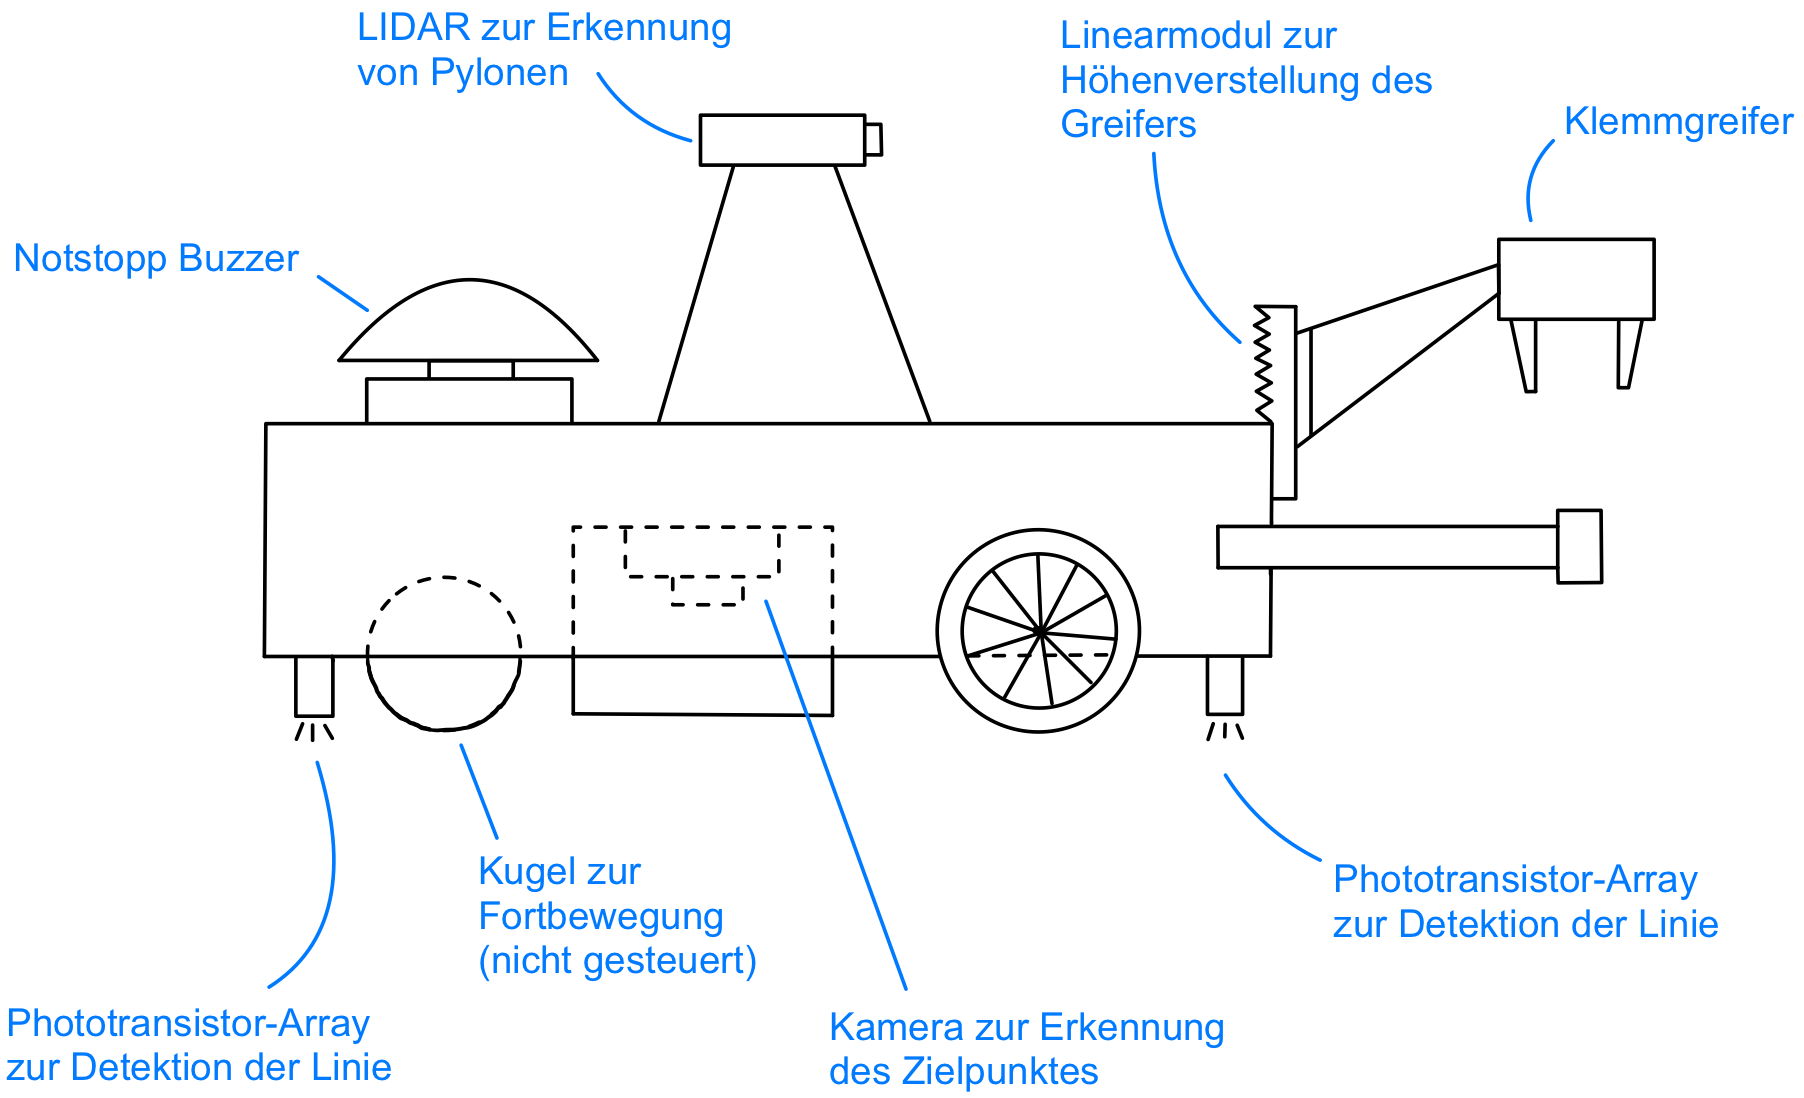
\includegraphics[width=1\textwidth]{./Skizzen/Sketch_Side.png} % Adjust the width to 50% of text width
        \caption{Seitenansicht rote Variante} % Caption for the figure
        \label{fig:Sketch_Side} % Label for referencing the figure
    \end{figure}

    \newpage

    \begin{figure}[h] % 'h' means here, placing the figure at the location in the text
        \centering % Center the figure on the page
        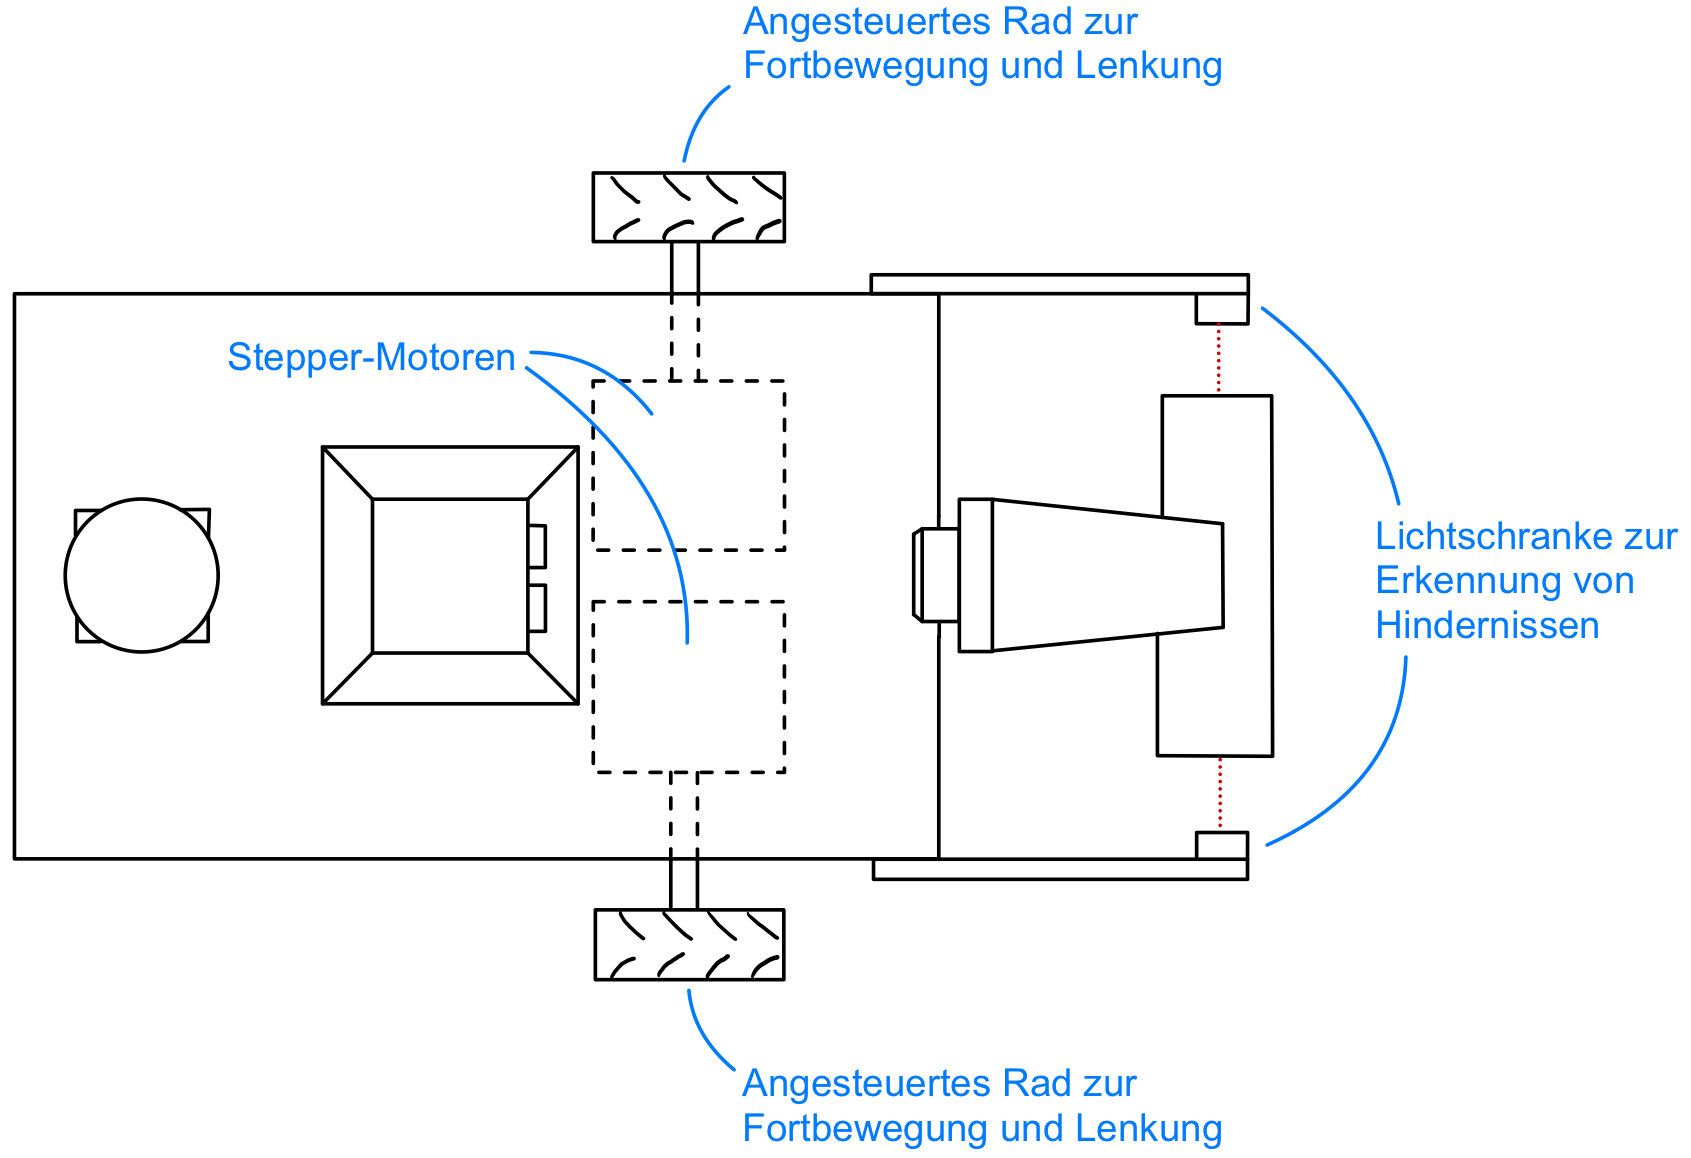
\includegraphics[width=1\textwidth]{./Skizzen/Sketch_Top.png} % Adjust the width to 50% of text width
        \caption{Draufsicht rote Variante} % Caption for the figure
        \label{fig:Sketch_Top} % Label for referencing the figure
    \end{figure}

\end{landscape} % Querformat beenden

\end{document}
